%--------------------------------------
%	PAKET-/ UND ANDERE DOKUMENT-IMPORTS
%--------------------------------------
\documentclass{scrartcl}   % Formateinstellungen
\usepackage[ngerman]{babel} % deutsche Silbentrennung
\usepackage[utf8]{inputenc} % deutsche Umlaute
\usepackage{placeins}   % verbessert Anzeige eines Floats hinter dem Befehl \FloatBarrier
\usepackage{amsfonts}   % neue Schriftanpassungen (wird von amssymb (s.u.) geladen)
\usepackage{amssymb}    % erweitert Benutzung von amsfonts (s.o.)
\usepackage{amsmath}    % Vielzahl von neuen mathematischen Umgebungen und Befehlen (wird von mathtools (s.u.) geladen)
\usepackage{mathtools}  % Verbesserung von amsmath (s.o.)
\usepackage{booktabs}   % Tabellen ohne vertikale Striche
\usepackage{siunitx}    % Einheitensystem
\usepackage[margin={0.3cm,0.3cm},font=singlespacing,labelfont=bf,labelsep=endash]{caption} % Bildunterschriften
\usepackage{wrapfig}    % Bild von Text umfließen lassen
\usepackage{sidecap}    % ermöglicht Überschriften neben Bildern / Tabellen
\usepackage{setspace}   % zum Definieren des Zeilenabstandes
\usepackage{eurosym}    % ergänzt optimales Euro-Zeichen
\usepackage[perpage,marginal]{footmisc} % ermöglicht Fußnoten und das Verändern dieser
\usepackage{graphicx}   % ermöglicht besseres Einbinden von Grafiken
\usepackage{fancyhdr}   % zum Erstellen von Kopf- und Fußzeilen
\usepackage{listings}   % ermöglicht Quellcodelisting
\usepackage{color}  % Farb-Management von Vorder- und Hintergrundfarben
\usepackage{pdfpages}   % ermöglicht das Einbinden von ganzen oder nur Teilen von PDFs
\usepackage{lineno} % Zeilenzählung
\usepackage{framed} % ermöglicht das Einrahmen von Elementen
\usepackage{pifont} % fügt Symbol-Schriften hinzu
\usepackage[hidelinks]{hyperref}    % ermöglicht das Hinzufügen von Links und Verweisen innerhalb
                                    % des PDF Dokuments und weitere Einstellungen
\usepackage[left=2.5cm,right=2cm,top=2cm,bottom=2cm,includeheadfoot]{geometry}  % Größenanpassung der Seite
%--------------------------------------


%--------------------------------------
%   KONFIGURATIONEN
%--------------------------------------
\begin{document}
\setlength{\parskip}{1ex}   % Abstand zwischen Absätzen 
\parindent 0pt  % legt Einrücke der ersten Zeile fest
\renewcommand{\thefigure}{\arabic{figure}.\alph{ab}}    % Umdefinieren von Bildnummern

\definecolor{darkblue}{rgb}{0,0,.6} % Festlegen der Farben
\definecolor{darkred}{rgb}{.6,0,0}  % Festlegen der Farben
\definecolor{darkgreen}{rgb}{0,.6,0}    % Festlegen der Farben
\definecolor{red}{rgb}{.98,0,0} % Festlegen der Farben

\lstloadlanguages{Java} % lädt Programmiersprachen
\lstset{language=Java,basicstyle=\footnotesize\ttfamily,commentstyle=\itshape\color{darkgreen},keywordstyle=\bfseries\color{darkblue},stringstyle=\color{darkred},tabsize=3,showspaces=false,showtabs=false,columns=fixed,numbers=left,frame=single,numberstyle=\tiny,breaklines=true,showstringspaces=false,xleftmargin=1cm} % Erstellen eines Codeblocks
    
\pagestyle{fancy}   % Setzen des Seitenstyles "fancy" ermöglicht eigenes Erstellen einer Kopf- und Fußzeile
\fancyhf{}  % alle Kopf- und Fußzeilenfelder bereinigen
\fancyhead[L]{\leftmark}    % Kopfzeile links (mit "leftmark" erstellt man im Header das Chapter, mit "rightmark" die Section)
\fancyhead[C]{} % zentrierte Kopfzeile
\fancyhead[R]{\thepage} % Kopfzeile rechts
\fancypagestyle{plain}  % legt Seiten-Typen fest

\newcommand{\barrow}{\item[\ding{228}]} % hinzufügen des Pfeil-Aufzählsymbols unter dem Command \barrow
%--------------------------------------


%--------------------------------------
%   1. SEITE
%--------------------------------------
\titlehead{\Large

\begin{center}
\centering 
\begin{normalsize}
\textit{Lizensiert unter einer \href{https://creativecommons.org/licenses/by-sa/4.0/legalcode.de}{CC-BY-SA 4.0-Lizenz}}
\end{normalsize}
\begin{framed}
\centering {Inoffizielle Lösungen und Erklärungen - \href{https://www.inf-schule.de}{inf-schule} (\href{https://creativecommons.org/licenses/by-sa/4.0/legalcode.de}{\textit{Lizenz}})}

\centering {\Large\textbf{\href{https://www.inf-schule.de/oop/java}{7.1 Objektorientierte Programmierung mit Java}}}
\end{framed}
\end{center}}

\title{\huge{\href{https://www.inf-schule.de/oop/java/implementierung/siw}{2.2\\Schweine im Weltall}}\\
\vspace{0.5cm}
\begin{figure}[ht]
	\centering
	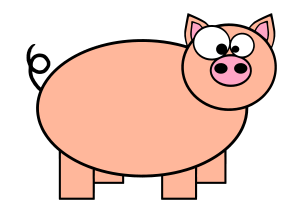
\includegraphics[height=4.5cm]{Schweine_im_Weltall.png}
\end{figure}
\vspace{0.7cm}}

\author{\textbf{Benötigte IDEs:}\\
\href{https://www.greenfoot.org/}{Greenfoot}, \href{https://www.bluej.org/}{BlueJ}
\vspace{1cm}}

\date{\textbf{Verfasser:}\\
\href{https://cyb3rko.de}{Niko Diamadis (Cyb3rKo)}\\
\vspace{1cm}
\textbf{Erstellungs-/ Änderungsdatum}\\
\today\enlargethispage{4cm}}
%--------------------------------------

%--------------------------------------
%   2. SEITE
%--------------------------------------
\doublespacing

\maketitle\thispagestyle{empty}

\numberwithin{equation}{section}
\cleardoublepage

\setcounter{page}{1}
\tableofcontents
%--------------------------------------


%--------------------------------------
%   3. UND NACHFOLGENDE SEITEN
%--------------------------------------
\newpage
\pagenumbering{arabic}  % Ändern der Seitenangabe

\cleardoublepage

\section{Implementierung des Grundgerüsts}

\subsection{Projekt vorbereiten}

Das Schwein kann bereits Methoden ausführen, auch wenn wir noch nichts programmiert haben, denn da das Schwein eine Unterklasse von \texttt{Actor} ist, übernimmt es automatisch alle Attribute und Methoden aus der Oberklasse.

\subsection{Erste Bewegungen}

\begin{lstlisting}
public void act() {
    move(2);
    turn(2);
}
\end{lstlisting}

\subsection{Zufällige Bewegungen}

\begin{figure}[ht]
	\centering
	\includegraphics[height=5.5cm]{7.1.2.2/1.Implementierung_des_Grundgeruestes/3-1.jpg}
\end{figure}

Nicht verwirren lassen, wenn man nur eine Zeile an Code in der if- bzw. else-Schleife stehen hat, können die geschweiften Klammern weggelassen werden. Ich benutze sie jedoch IMMER...

\newpage

\subsection{Nicht so zappelig}

\begin{figure}[ht]
	\centering
	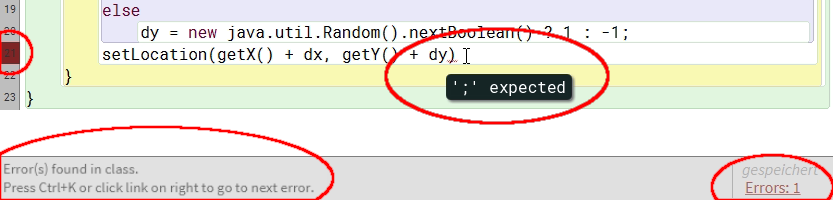
\includegraphics[height=13cm]{7.1.2.2/1.Implementierung_des_Grundgeruestes/4-1.png}
\end{figure}

\begin{figure}[ht]
	\centering
	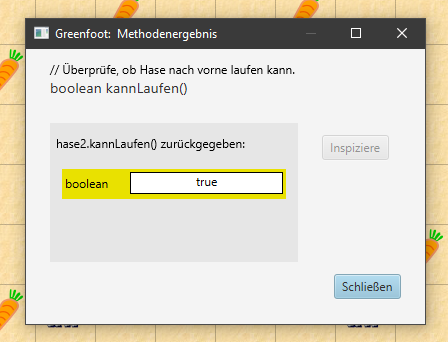
\includegraphics[height=5cm]{7.1.2.2/1.Implementierung_des_Grundgeruestes/4-2.png}
\end{figure}

\newpage

\begin{lstlisting}
public void act() {
    move(2);
    
    int zufallszahl = new java.util.Random().nextInt(20);
    
    if (zufallszahl == 0) {
        turn(20);
    } else if (zufallszahl == 1) { 
        turn(-20);
    }
}    
\end{lstlisting}

Wenn die Zufallszahl im Bereich von 2 bis 19 liegt passiert nichts. Innerhalb der \texttt{act}-Methode wird dann also nur \texttt{move(2)} aufgerufen.\\
Wir haben jetzt eine Wahrscheinlichkeit von 20\%, dass sich das Schwein bewegt, es dreht sich dann jedoch mehr als vorher.

So können wir die zittrige Bewegung vermeiden.

\subsection{Spielende auf Mausklick}

Folgender Code muss einfach in der \texttt{act}-Methode zum restlichen Code hinzufügt werden.\\
\begin{lstlisting}
if (Greenfoot.mouseClicked(this)) {
    Greenfoot.playSound("pig.wav");
    Greenfoot.stop();
}
\end{lstlisting}

\newpage

\subsection{Altes Schwein}

Da nun auch ein Attribut hinzugefügt werden muss, hier nun der ganze Code der Klasse:\\
\begin{lstlisting}
import greenfoot.*;

public class Schwein extends Actor {
    int alter;
    
    public void act() {
        alter++;
        
        if (alter == 1000) {
            setImage("boom.png");
            Greenfoot.stop();
        }
        
        if (Greenfoot.mouseClicked(this)) {
            Greenfoot.playSound("pig.wav");
            Greenfoot.stop();
        }
        
        move(2);
        
        int zufallszahl = new java.util.Random().nextInt(20);
        
        if (zufallszahl == 0) {
            turn(20);
        } else if (zufallszahl == 1) { 
            turn(-20);
        }
    }    
}
\end{lstlisting}

\newpage

\subsection{Spiel vorbereiten}

Wenn ihr die beschriebenen Schritte befolgt habt, findest du den Code zum automatischen Erzeugen des Schweins in der Welt-Unterklasse \texttt{PigWorld}.\\
\begin{lstlisting}
public PigWorld() {    
    super(600, 450, 1); 
    prepare();
}

private void prepare() {
    Schwein schwein = new Schwein();
    addObject(schwein,303,227);
}
\end{lstlisting}

Wie hoffentlich zu erkennen ist, wird im Konstruktor die Methode \texttt{prepare} aufgerufen, welche eben für das Erzeugen des Schweins verantwortlich ist.

In der Methode wird ein neues Objekt der Klasse \texttt{Schwein} erzeugt mit dem Namen \texttt{schwein.}\\
Anschließend wird das Objekt in die Welt gesetzt, in meinem Falle auf die Koordinaten\\
$x=303$; $y=227$.

\newpage

\section{Fachkonzept - Vererbung}

Zu dieser Seite sind meines Erachtens nach keine Anleitungen und/oder Erläuterungen nötig.\\
Wenn doch Fragen aufkommen, schreib' einfach an \textbf{\href{mailto:niko@cyb3rko.de}{niko@cyb3rko.de}}.

\newpage

\section{Fachkonzept - Klassenmethoden}

Zu dieser Seite sind meines Erachtens nach keine Anleitungen und/oder Erläuterungen nötig.\\
Wenn doch Fragen aufkommen, schreib' einfach an \textbf{\href{mailto:niko@cyb3rko.de}{niko@cyb3rko.de}}.

\newpage

\section{Übungen}

\subsection{Zufällig Springen}

Um herauszufinden, wie das Schwein ermitteln kann, ob es den Rand berührt, gucken wir uns an, welche Methoden es geerbt hat.\\
Dazu klickt man mit einem Rechtsklick auf das Schwein und geht über \texttt{geerbt von ...} .

Beim Durchsehen der Methoden stößt man auf die Methode \texttt{isAtEdge} mit boolean als Rückgabewert. Das ist genau das Richtige für uns.\\

\begin{figure}[ht]
	\centering
	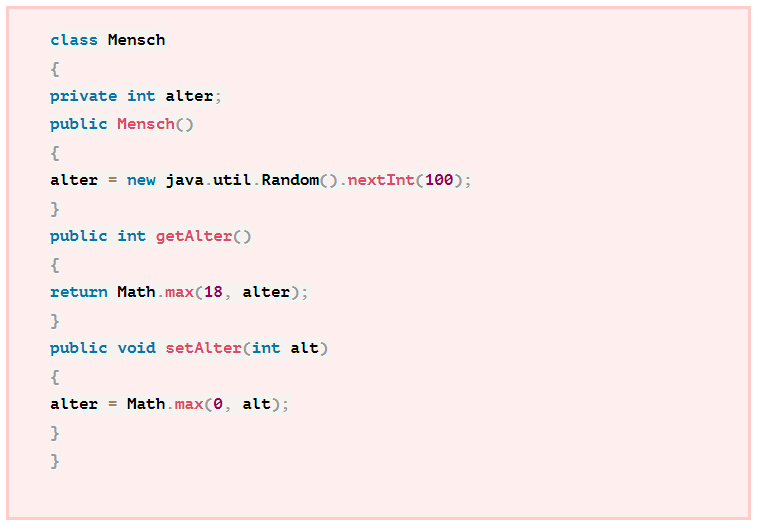
\includegraphics[height=12cm]{7.1.2.2/4.Uebungen/1-1.png}
\end{figure}

Wir wollen also, wenn das Schwein am Ende der Welt ist, es auf eine zufällige Position setzen.\\
Als passende Methode findet man \texttt{setLocation} mit zwei Parametern, und zwar der x- und y-Koordinate.

\newpage

Implementiert sieht das dann z.B. so aus:\\
\begin{lstlisting}
if (isAtEdge()) {
    setLocation(Greenfoot.getRandomNumber(600), Greenfoot.getRandomNumber(450));
}
\end{lstlisting}

Bitte nicht wundern, die Zeile war zu lang für das Dokument, deshalb ist ein Zeilensprung eingebaut worden, es gehört aber alles ein eine Zeile.\\

Die Breite und Höhe der Welt kann man aus dem Konstruktor der \texttt{PigWorld} ablesen.\\

\begin{figure}[ht]
	\centering
	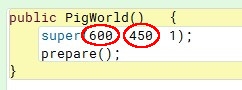
\includegraphics[height=3.5cm]{7.1.2.2/4.Uebungen/1-2.jpg}
\end{figure}

\subsection{Aus der Welt laufen}

Der Programmierer wollte wohl erreichen, dass das Schwein bei Berühren des Endes der Welt auf die andere Seite gesetzt wird.

Jedoch gibt es da ein Problem:\\
Wenn das Schwein z.B. bei $x=0$ ist, ist die erste Bedingung erfüllt und es wird auf \texttt{(599, getY())} gesetzt.\\
Anschließend wird jedoch überprüft, ob es bei $x=599$ ist. Da dies auch erfüllt ist, wird es wieder zurück auf $x=0$ gesetzt.

Um dieses Problem zu lösen, könnte man die vier if-Bedingungen in zwei if-/else if-Schleifen schreiben.

\begin{lstlisting}
if (getX() == 0) {
    setLocation(599, getY());
} else if (getX() == 599) {
    setLocation(0, getY());
}

if (getY() == 0) {
    setLocation(getX(), 449);
} else if (getY() == 449) {
    setLocation(getX(), 0);
}
\end{lstlisting}

In eine Schleife dürfte man nämlich nicht alle vier schreiben, da so z.B. der Fall augeschlossen wird, wenn das Schwein bei \texttt{x == 0} und \texttt{y == 0} ist.

\newpage

\subsection{Gewinnstufen}

Ich nehme wieder das \texttt{alter}-Attribut zur Hilfe.\\
Ich habe in diesem Fall eine Fallunterscheidung in 250er-Schritten eingebaut, die nach Klicken des Schweins folgendermaßen aussieht:\\

\begin{figure}[ht]
	\centering
	\includegraphics[height=10cm]{7.1.2.2/4.Uebungen/3-1.png}
\end{figure}

Der Vorteil eines Struktogramms ist, dass die Blockform eine ordentliche Anschauung ermöglicht und der Ablauf der Aktionen eindeutig ist, Nachteil ist die unklarere Darstellung verschiedener Elemente und dass ein Struktogramm innerhalb weniger Schritte sehr breit werden kann.\\

\newpage

Im Vergleich dazu das Flussdiagramm:

\begin{figure}[ht]
	\centering
	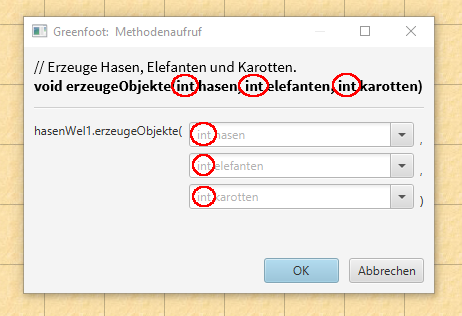
\includegraphics[height=14cm]{7.1.2.2/4.Uebungen/3-2.png}
\end{figure}

Bei Flussdiagrammen ist der Ablauf der Aktionen unklarer, da Pfeile bei Wiederholungen wieder zum Anfang oder zu anderen Elementen weiter am Ende verweisen können, jedoch ist dort klarer zu erkennen, um welche Art von Element es geht (z.B. while-Schleife, for-Schleife, if-Bedingung, ...).\\
Außerdem ist es leichter, die Form anzupassen, falls das Diagramm zu breit, zu groß oder zu hoch erscheint.\\

\newpage

Die Bilder findet man im Projektordner im Unterordner \texttt{images}.\\

\begin{figure}[ht]
	\centering
	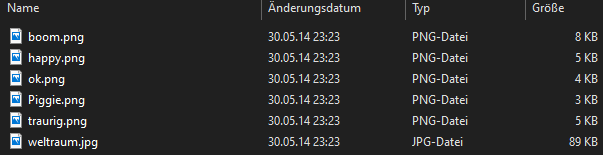
\includegraphics[height=4cm]{7.1.2.2/4.Uebungen/3-3.png}
\end{figure}

Implementiert sieht der Code anschließend z.B. so aus:

\begin{lstlisting}
if (Greenfoot.mousePressed(this)) {
    if (alter < 250) {
        setImage("boom.png");
    } else if (alter > 249 && alter < 500) {
        setImage("traurig.png");
    } else if (alter > 499 && alter < 750) {
        setImage("ok.png");
    } else if (alter > 749) {
        setImage("happy.png");
    }
    
    setRotation(0);
    Greenfoot.stop();
    Greenfoot.playSound("pig.wav");
}
\end{lstlisting}

\newpage

\subsection{Eigene Ideen}

In dieser Aufgabe werde ich einfach nur die Beispiele verwirklichen, du kannst hier deine eigenen Ideen verwirklichen.

\begin{itemize}
    \barrow
    \begin{lstlisting}
int drehzahl;

public void act() {
    ...

    int zufallszahl = new java.util.Random().nextInt(2);
    
    drehzahl++;

    if (drehzahl == 20) {
        if (zufallszahl == 0) {
            turn(20);
        } else    {
            turn(-20);
        }
        
        drehzahl = 0;
    }
    
    ...
}
    \end{lstlisting}
    \barrow Für zufällige Geschwindigkeit nutzen wir die implementierte Variable \texttt{zufallszahl} erneut.
    \begin{lstlisting}
zufallszahl = new java.util.Random().nextInt(20);
    
if (zufallszahl == 0) {
    Greenfoot.setSpeed(50);
} else if (zufallszahl == 1) {
    Greenfoot.setSpeed(55);
}
    \end{lstlisting}
    \barrow Ich habe im Beispiel festgelegt, dass bei Fehlklick das Schwein zufällig ein wenig an der x- und y-Achse verschoben wird.\\
    \begin{lstlisting}
if (Greenfoot.mousePressed(this)) {
    ...
} else if (Greenfoot.mousePressed(getWorld())) {
    int zufallszahl1 = new java.util.Random().nextInt(100) - 50;
    int zufallszahl2 = new java.util.Random().nextInt(100) - 50;
    
    setLocation(getX() + zufallszahl1, getY() + zufallszahl2);
}
    \end{lstlisting}
    Ich habe zwei Hilfsvariablen benutzt, da ohne diese die Zeile (welche anfängt mit \texttt{setLocation(...)}) zu lang und unübersichtlich werden würde.\\
    Das \text{getWorld()} in der Bedingung ruft die Methode \texttt{getWorld} auf, welche die Welt zurückgibt, wodurch man die Methode wie ein Objekt benutzen kann.\\
\end{itemize}

Mit allen Änderungen und Neuerungen sieht die ganze Klasse nun so aus:

\begin{lstlisting}
import greenfoot.*;

public class Schwein extends Actor {
    int alter;
    int drehzahl;

    public void act() {
        if (Greenfoot.mousePressed(this)) {
            if (alter < 250) {
                setImage("boom.png");
            } else if (alter > 249 && alter < 500) {
                setImage("traurig.png");
            } else if (alter > 499 && alter < 750) {
                setImage("ok.png");
            } else if (alter > 749) {
                setImage("happy.png");
            }

            setRotation(0);
            Greenfoot.stop();
            Greenfoot.playSound("pig.wav");
        } else if (Greenfoot.mousePressed(getWorld())) {
            int zufallszahl1 = new java.util.Random().nextInt(100) - 50;
            int zufallszahl2 = new java.util.Random().nextInt(100) - 50;
            
            setLocation(getX() + zufallszahl1, getY() + zufallszahl2);
        }

        if (getX() == 0) {
            setLocation(599, getY());
        } else if (getX() == 599) {
            setLocation(0, getY());
        }

        if (getY() == 0) {
            setLocation(getX(), 449);
        } else if (getY() == 449) {
            setLocation(getX(), 0);
        }

        move(2);

        int zufallszahl = new java.util.Random().nextInt(2);

        drehzahl++;

        if (drehzahl == 20) {
            if (zufallszahl == 0) {
                turn(20);
                
            } else {
                turn(-20);
            }

            drehzahl = 0;
        }

        zufallszahl = new java.util.Random().nextInt(20);

        if (zufallszahl == 0) {
            Greenfoot.setSpeed(50);
        } else if (zufallszahl == 1) {
            Greenfoot.setSpeed(55);
        }

        alter++;
    }
}
\end{lstlisting}

\subsection{Mathematische Funktionen}

Wahrscheinlich haben die Java-Entwickler sich dazu entschieden, da man durch Benutzung von Klassenmethoden das Erstellen von Objekten vermeiden kann.

Ein Objekt der Klasse \texttt{Math} würde meistens auch keinen Sinn machen.

\newpage

\subsection{GeoCalc}

\begin{itemize}
    \item[\textbf{a.}] Zum einen gibt es die Klasse \texttt{Geofigur} mit mehreren Attributen und Methoden.\\
    Des Weiteren gibt es die Klasse \texttt{Rechteck}, Unterklasse von \texttt{Geofigur}, welcher alle Variablen und Methoden von \texttt{Geofigur} \textit{vererbt} wurden.
    
    Die in \texttt{Rechteck} implementierten Attribute und Methoden werden zu den vererbten Variablen und Methoden \textit{ergänzt}. Als Ausnahme ist zu erwähnen, dass \textit{Vererbtes} \textit{überschrieben} wird, falls in der Unterklasse Variablen bzw. Methoden mit demselben Namen neu implementiert werden.
    
    \item[\textbf{b.}] Zur Berechnung des Abstandes habe ich den Satz des Pythagoras benutzt:
    \begin{figure}[ht]
    	\centering
    	$a^2 + b^2 = c^2$
    \end{figure}
    
    \texttt{a} ist in unserem Falle \texttt{x} + die Hälfte der Breite, \texttt{b} ist \texttt{y} + die Hälfte der Höhe, da wir ja den Abstand zwischen Ursprung und Mittelpunkt des Rechtecks errechnen möchte.\\
    Zum Ausrechnen nehmen wir also die Quadratwurzel aus dem Quadrat von \texttt{a} und dem Quadrat aus \texttt{b}.\\
    \begin{lstlisting}
class Rechteck extends GeoFigur {
    double breite;
    double hoehe;
    
    void setzeAusmasse(double b, double h) {
        breite = b;
        hoehe = h;
    }
    
    double getFlaeche() {
        return breite * hoehe;
    }
    
    
    
    
    double getAbstandZumUrsprung() {
        return Math.sqrt(Math.pow(x + breite / 2, 2) + Math.pow(y + hoehe / 2, 2));
    }
}
    \end{lstlisting}
    \item[\textbf{c.}] Zu dieser Aufgabe sind meines Erachtens nach keine Anleitungen und/oder Erläuterungen nötig.\\
Wenn doch Fragen aufkommen, schreib' einfach an \textbf{\href{mailto:niko@cyb3rko.de}{niko@cyb3rko.de}}.
    \item[\textbf{d.}]
    \begin{itemize}
        \barrow \textbf{1. Zeile}\\
        Es wird ein Objekt \texttt{figur} der Klasse \texttt{GeoFigur} erstellt.
        \barrow \textbf{2. Zeile}\\
        Am Objekt \texttt{figur} wird die Methode \texttt{setzeKoordinaten} mit den Parametern \texttt{0} und \texttt{2} aufgerufen, für \texttt{x} wird also \texttt{0} und für \texttt{y} wird \texttt{2} gesetzt.
        \barrow \textbf{3. Zeile}\\
        Es wird der Rückgabewert der Methode \texttt{getAbstandZumUrsprung} vom Objekt \texttt{figur} in der Konsole ausgegeben.
        \barrow \textbf{4. Zeile}\\
        Es wird ein Objekt \texttt{rechteck} der Klasse \texttt{Rechteck} erstellt.
        \barrow \textbf{5. Zeile}\\
        Am Objekt \texttt{rechteck} wird die Methode \texttt{setzeKoordinaten}, welche von der Klasse \texttt{GeoFigur} vererbt wurde, mit den Parametern \texttt{-2} und \texttt{2} aufgerufen, für \texttt{x} wird also \texttt{-2} und für \texttt{y} wird \texttt{2} gesetzt.
        \barrow \textbf{6. Zeile}\\
        Am Objekt \texttt{rechteck} wird die Methode \texttt{setzeAusmasse} mit den Parametern \texttt{4} und \texttt{4} aufgerufen, für \texttt{breite} wird also \texttt{4} und für \texttt{hoehe} wird auch \texttt{4} gesetzt.
        \barrow \textbf{7. Zeile}\\
        Am Objekt \texttt{rechteck} wird die Methode \texttt{verschieben}, welche von der Klasse \texttt{GeoFigur} vererbt wurde, mit den Parametern \texttt{0} und \texttt{2} aufgerufen, \texttt{x} bleibt also gleich und für \texttt{y} wird von \texttt{4} nun zu \texttt{6} geändert.
        \barrow \textbf{8. Zeile}\\
        Es wird der Rückgabewert der Methode \texttt{getAbstandZumUrsprung} vom Objekt \texttt{rechteck} in der Konsole ausgegeben.
        \barrow \textbf{\textcolor{darkred}{9. Zeile}}\\
        Es wird ein Objekt \texttt{g} der Klasse \texttt{GeoFigur} erstellt, jedoch mithilfe des Konstruktors der Klasse \texttt{Rechteck}, was erstmal keinen Fehler beim Compilieren hervorruft, da ein Rechteck, welches durch den Konstruktor aufgerufen wird, in eine GeoFigur verwandelt werden kann, da es eine Unterklasse ist, uns aber in den nächsten Schritten Probleme bereiten wird.
        \barrow \textbf{10. Zeile}\\
        Am Objekt \texttt{g} wird die Methode \texttt{setzeKoordinaten} mit den Parametern \texttt{0} und \texttt{1} aufgerufen, für \texttt{x} wird also \texttt{0} und für \texttt{y} wird \texttt{1} gesetzt.
        \barrow \textbf{\textcolor{darkred}{11. Zeile}}\\
        Am Objekt \texttt{g} wird versucht, die Methode \texttt{setzeAusmasse} mit den Parametern \texttt{1} und \texttt{4} aufzurufen, aber da \texttt{g} in ein Objekt der Klasse \texttt{GeoFigur} umgewandelt worden ist, hat \texttt{g} keinen Zugriff auf eine Methode dieses Namens.\\
        Um das Problem zu lösen, könnte man in Zeile 9 \glqq GeoFigur\grqq{} durch \glqq Rechteck\grqq{} ersetzen. Zeile 10 wird keinen Fehler hervorrufen, da die Methode \texttt{setzeKoordinaten} auch wieder vererbt wird.
        \barrow \textbf{\textcolor{darkred}{12. Zeile}}\\
        Es wird versucht, ein Objekt \texttt{r} der Klasse \texttt{Rechteck} zu erstellen, jedoch mithilfe des Konstruktors der Klasse \texttt{GeoFigur}, was nicht funktioniert und eine Fehlermeldung hervorruft, da die GeoFigur, welche durch Aufruf des Konstruktors aufgerufen wird, nicht zurück in eine Unterklasse verwandelt werden kann.
    \end{itemize}
    
    \newpage
    
    \item[\textbf{e.}] Da beim Rechteck die gesamte Breite genommen wurde, habe ich mich beim Kreis für den Durchmesser entschieden. Zu beachten ist, dass jedoch mit dem Radius gerechnet wird.\\
    Die Koordinaten beschreiben die linke untere Ecke eines Quadrats, welches man anliegend an den Kreis um ihr herum zeichnen könnte.
    
    \begin{figure}[ht]
    	\centering
    	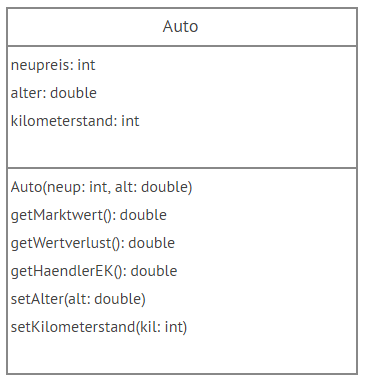
\includegraphics[height=11cm]{7.1.2.2/4.Uebungen/6-1.png}
    \end{figure}
    
    \begin{lstlisting}
class Kreis extends GeoFigur 
    double durchmesser;
    
    void setzeAusmasse(double durchmesser) {
        this.durchmesser = durchmesser;
    }
    
    double getFlaeche() {
        return Math.PI * Math.pow(durchmesser / 2, 2);
    }
    
    double getAbstandZumUrsprung() {
        return Math.sqrt(Math.pow(x + durchmesser / 2, 2) + Math.pow(y + durchmesser / 2, 2));
    }
}
    \end{lstlisting}
    
    \texttt{Math.PI} ist einfach nur genauer als 3,14. Zur Berechnung der Fläche habe ich die folgende Formel benutzt:
    \begin{figure}[ht]
    	\centering
    	$A = \pi r^2$\\
    \end{figure}
    \item[\textbf{f.}]
    \begin{itemize}
        \item[i.]
        \begin{lstlisting}
class Linie extends GeoFigur {
    double laenge;
    
    void setzeAusmasse(double laenge) {
        this.laenge = laenge;
    }
    
    double getAbstandZumUrsprung() {
        return Math.sqrt(Math.pow(x + laenge / 2, 2) + Math.pow(y, 2));
    }
    
    void skalieren(double faktor) {
        laenge *= faktor;
    }
}
        \end{lstlisting}
        \item[ii.]
        \begin{itemize}
        \barrow \textbf{Rechteck}
        \begin{lstlisting}
void skalieren(double faktor) {
    breite *= faktor;
    hoehe *= faktor;
}
        \end{lstlisting}
        
        \newpage
        
        \barrow \textbf{Kreis}
        \begin{lstlisting}
void skalieren(double faktor) {
    durchmesser *= faktor;
}
        \end{lstlisting}
        \barrow \textbf{Linie}
        \begin{lstlisting}
void skalieren(double faktor) {
    laenge *= faktor;
}
        \end{lstlisting}
    \end{itemize}
        \item[iii.]
        Nein, es macht keinen Sinn, denn alle Attribute und Methoden von \texttt{GeoFigur} sind ohne Probleme auch auf eine zweidimensionale Figur anzuwenden.\\
        Bei der Linie z.B. nimmt man als Koordinaten wieder den Punkt unten links an der Figur, der Mittelpunkt in die Mitte der Linie und den Abstand kann man dann auch berechnen.
    \end{itemize}
\end{itemize}

\end{document}